\chapter{Iteration 3 (FYP-2 Mid)}
\label{ch:iter3}
The first iteration is expected to be completed by the midterm of the FYP-2.
This chapter will have some of the artifacts based on system design. The requirements analysis section is same for all the systems while the design may vary. There may have two types of designs the structural design or . First section is for the structural design.
\section{FYP-2 Mid}
\textbf{Objectives for FYP-2 Mid}
	\begin{itemize}
		\item Basic tools
		\item Medicines 
		\item User movements
		\item Grabbing Tools
	\end{itemize}
\newpage
\subsection{Tools and Medicines}
\begin{figure}[h]
	\centering
	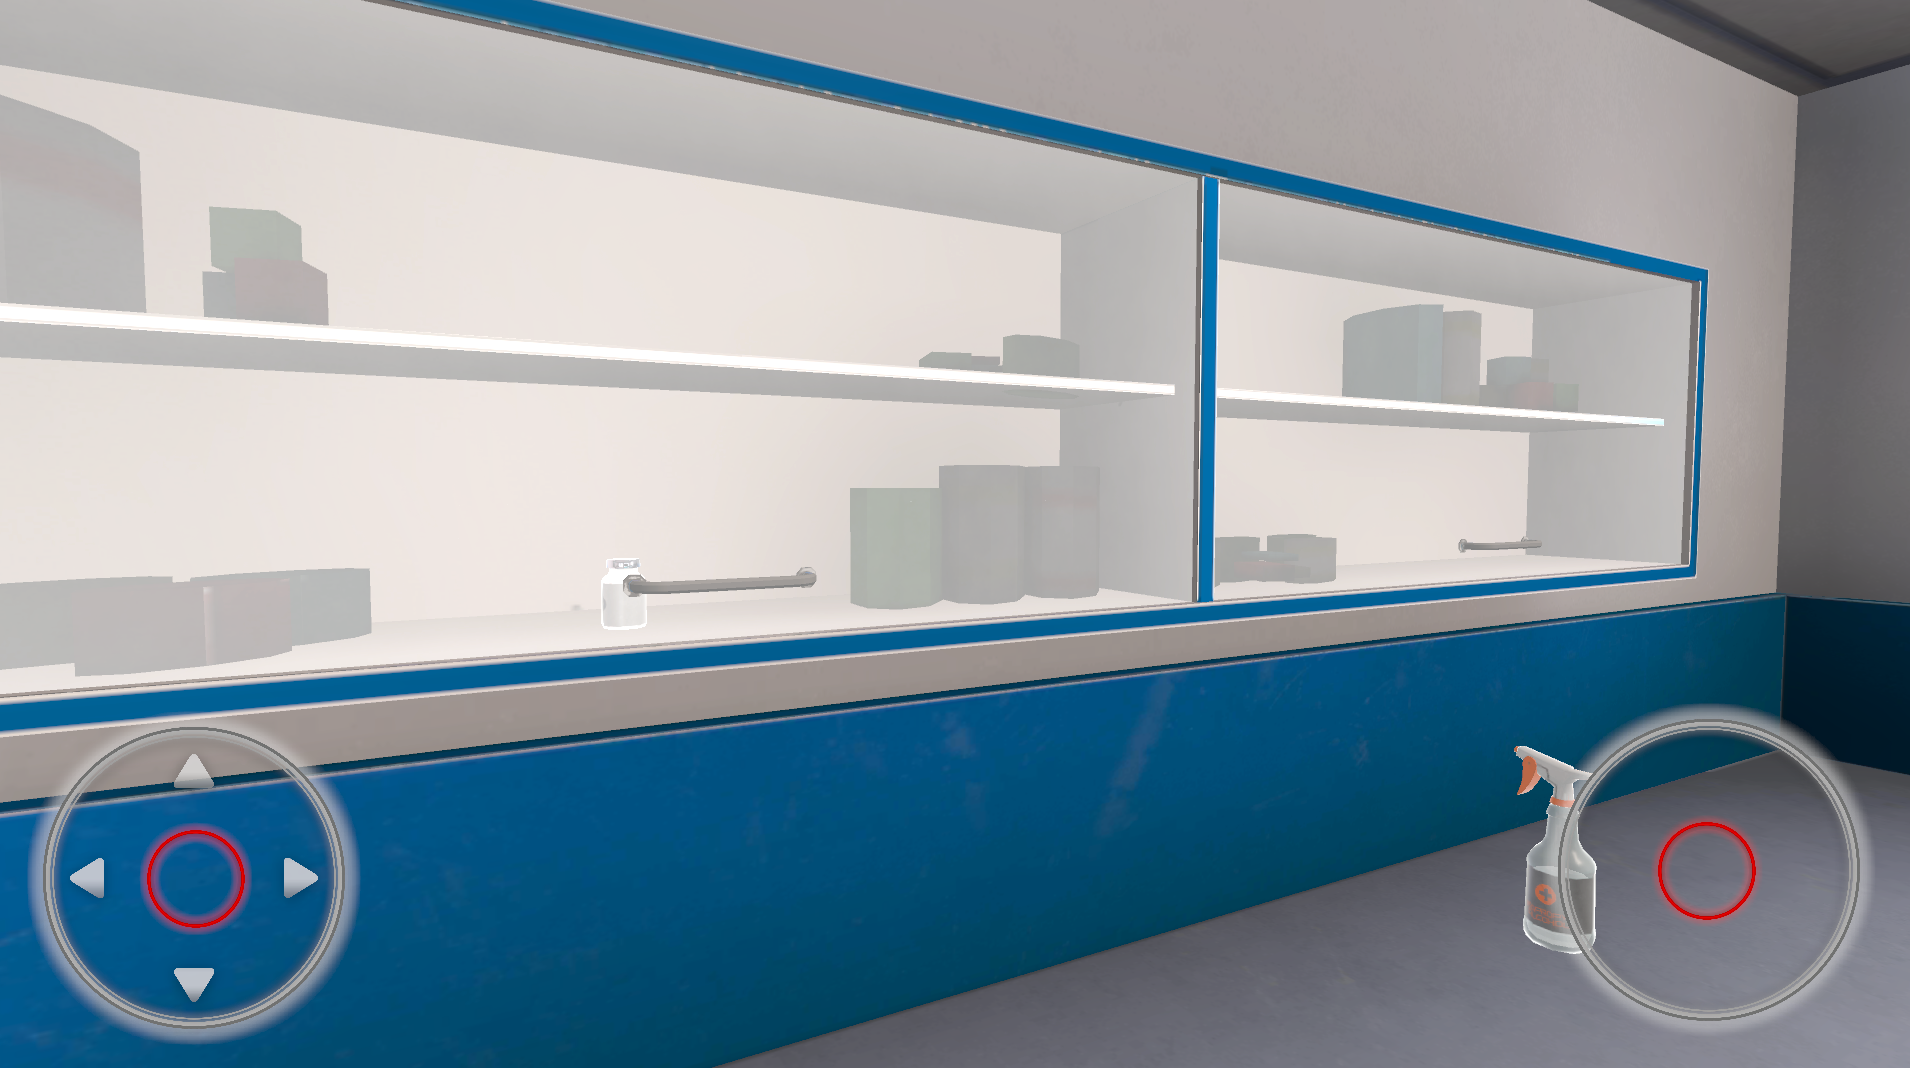
\includegraphics[width=0.7\textwidth, height=0.3\textheight]{Images/Tools and Medicine.png}
	\caption{Tools and Medicine box}
	\label{fig:Tools and Medicine}
\end{figure}

\subsection{Tools Grabbing}
\begin{figure}[h]
	\centering
	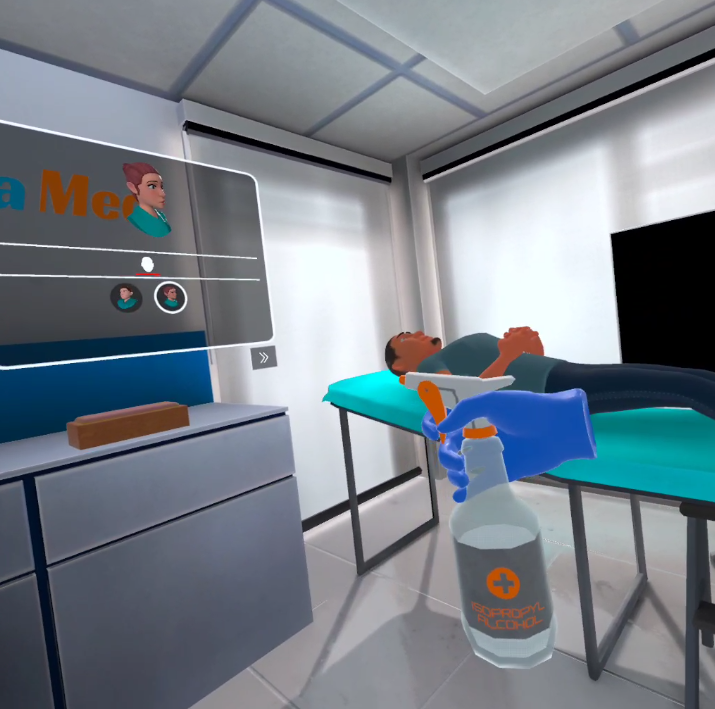
\includegraphics[width=0.7\textwidth, height=0.3\textheight]{Images/Grabbing Tool.png}
	\caption{Grabbing Tools}
	\label{fig:Grabbing Tools}
\end{figure}
\newpage
\subsubsection{Hands Washing}
\text{Here we are washing hand.}
\begin{figure}[h]
	\centering
     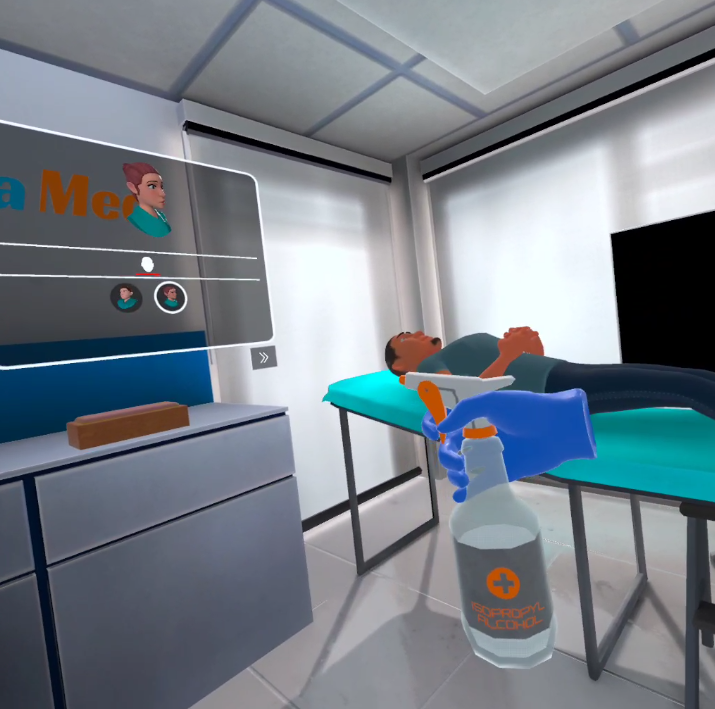
\includegraphics[width=0.7\textwidth, height=0.3\textheight]{Images/Washing hands.png}
	\caption{Hands Washing}
	\label{fig:Hands Washing}
\end{figure}

\subsubsection{Pour Alcohol}
\text{Here we are pouring alcohol to on cotton bud.}
\begin{figure}[h]
	\centering
	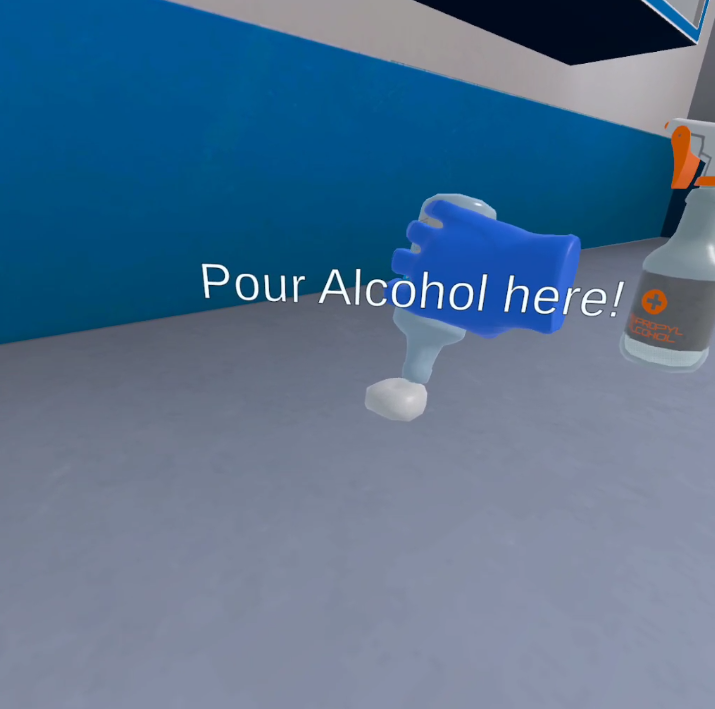
\includegraphics[width=0.7\textwidth, height=0.3\textheight]{Images/Pour Alcohol.png}
	\caption{Pour Alcohol}
	\label{fig:Pour-Alcohol}
\end{figure}
\newpage
\subsubsection{Clean the injection site}
\text{Here we are cleaning the injection site.}
\begin{figure}[h]
	\centering
	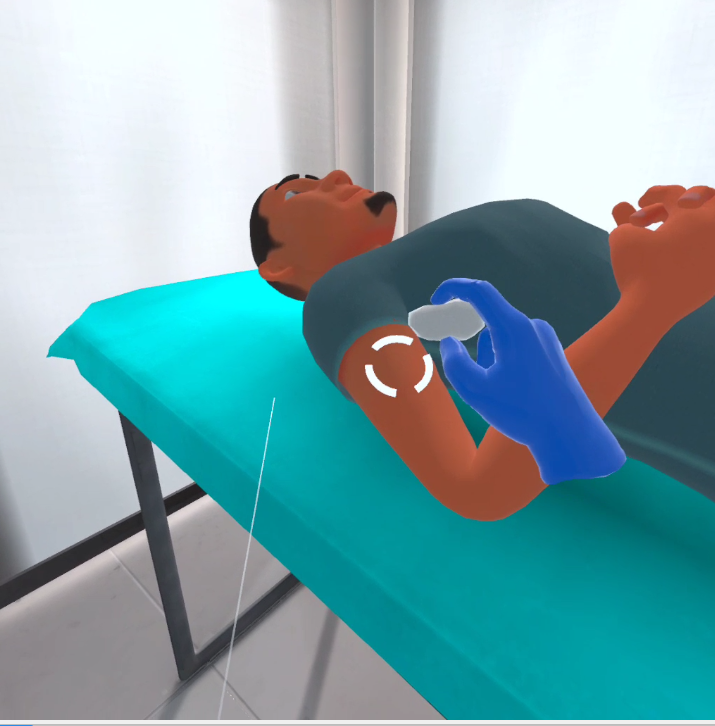
\includegraphics[width=0.7\textwidth, height=0.3\textheight]{Images/Clean the injection site.png}
	\caption{Clean the injection site}
	\label{fig:Clean the injection site}
\end{figure}
\subsubsection{Dispose the Cotton}
\text{Here we are disposing the cotton.}
\begin{figure}[h]
	\centering
	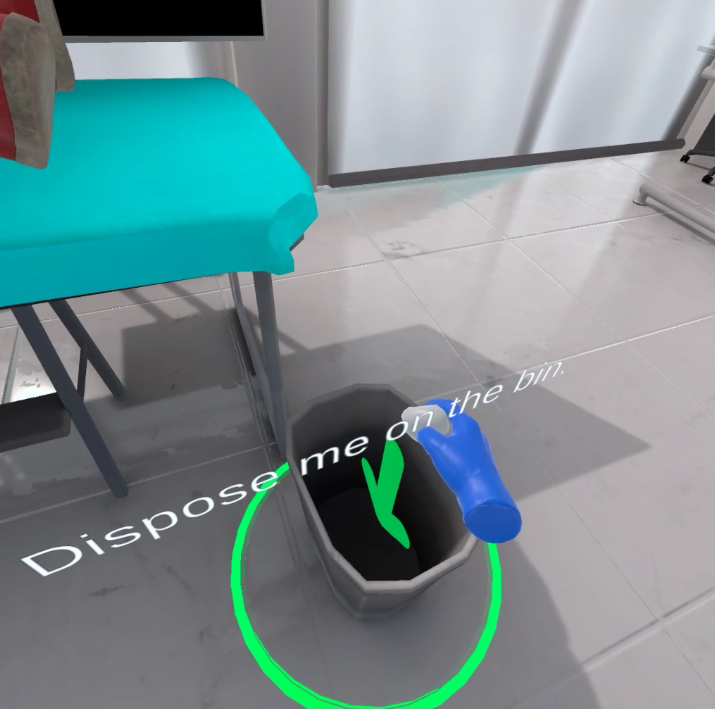
\includegraphics[width=0.7\textwidth, height=0.3\textheight]{Images/Dispose the Cotton.png}
	\caption{Dispose the Cotton}
	\label{fig:Dispose the Cotton}
\end{figure}
\newpage
\subsubsection{Picking the injection}
\text{Here we are picking the injection.}
\begin{figure}[h]
	\centering
	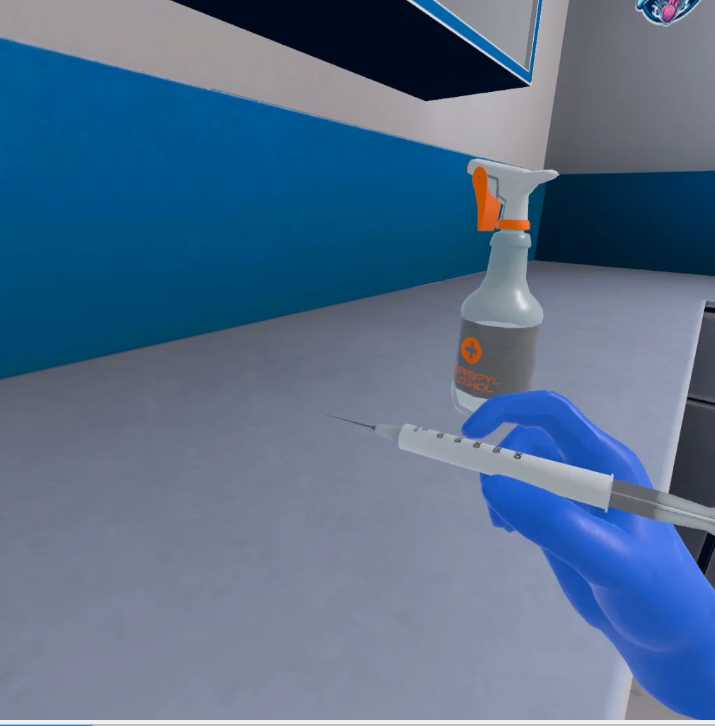
\includegraphics[width=0.7\textwidth, height=0.3\textheight]{Images/Picking the injection.png}
	\caption{Picking the injection}
	\label{fig:Picking the injection}
\end{figure}
\subsubsection{Inject the medication}
\text{Here we are inject the medication.}
\begin{figure}[h]
	\centering
	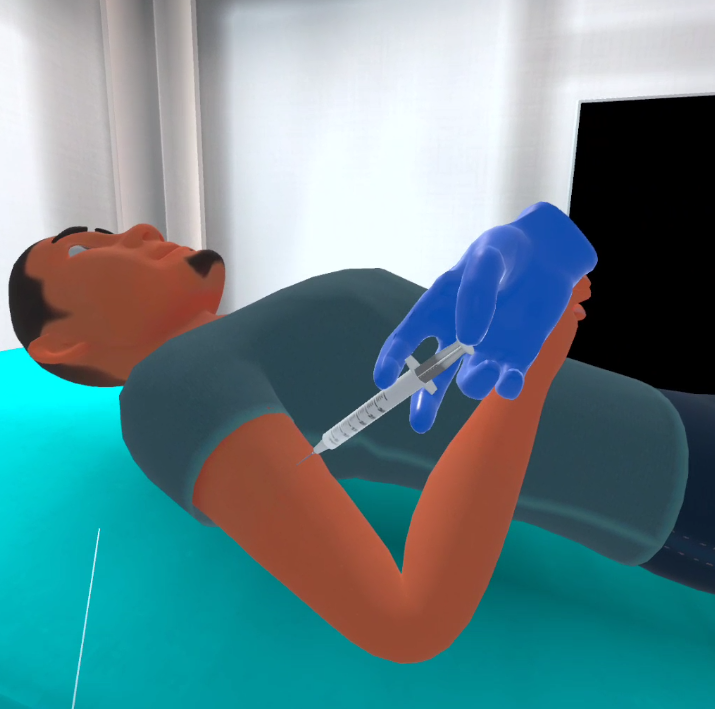
\includegraphics[width=0.7\textwidth, height=0.3\textheight]{Images/Inject the medication.png}
	\caption{Inject the medication}
	\label{fig:Inject the medication}
\end{figure}
\newpage
\subsubsection{Applying Cut on Body}
\text{Here we applying cut on body.}
\begin{figure}[h]
	\centering
	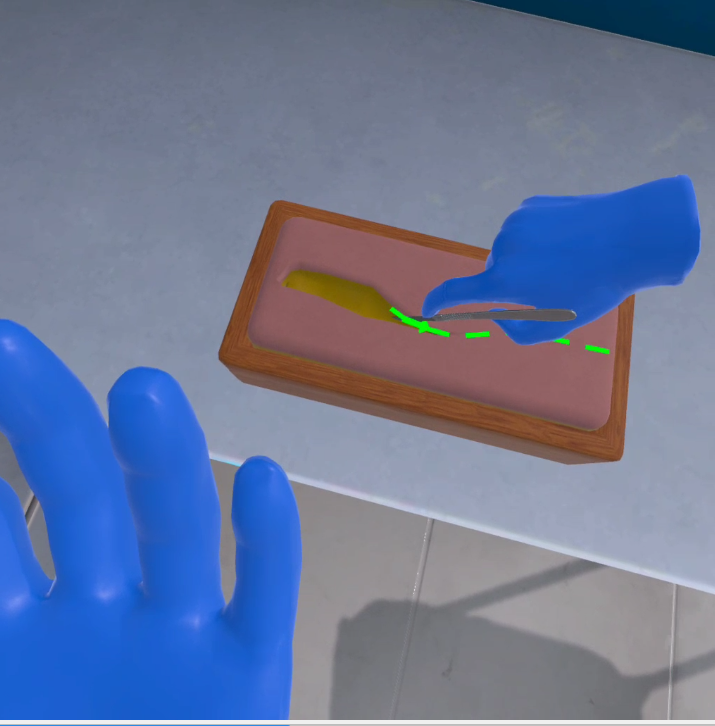
\includegraphics[width=0.7\textwidth, height=0.3\textheight]{Images/Applying Cut on Body.png}
	\caption{Applying Cut on Body}
	\label{fig:Applying Cut on Body}
\end{figure}
\newpage
\subsubsection{Objects Movement}
\text{Here are some code for actions performed by user.}
\text{User movement part 1 code.}
\newline
\begin{figure}[h]
	\centering
	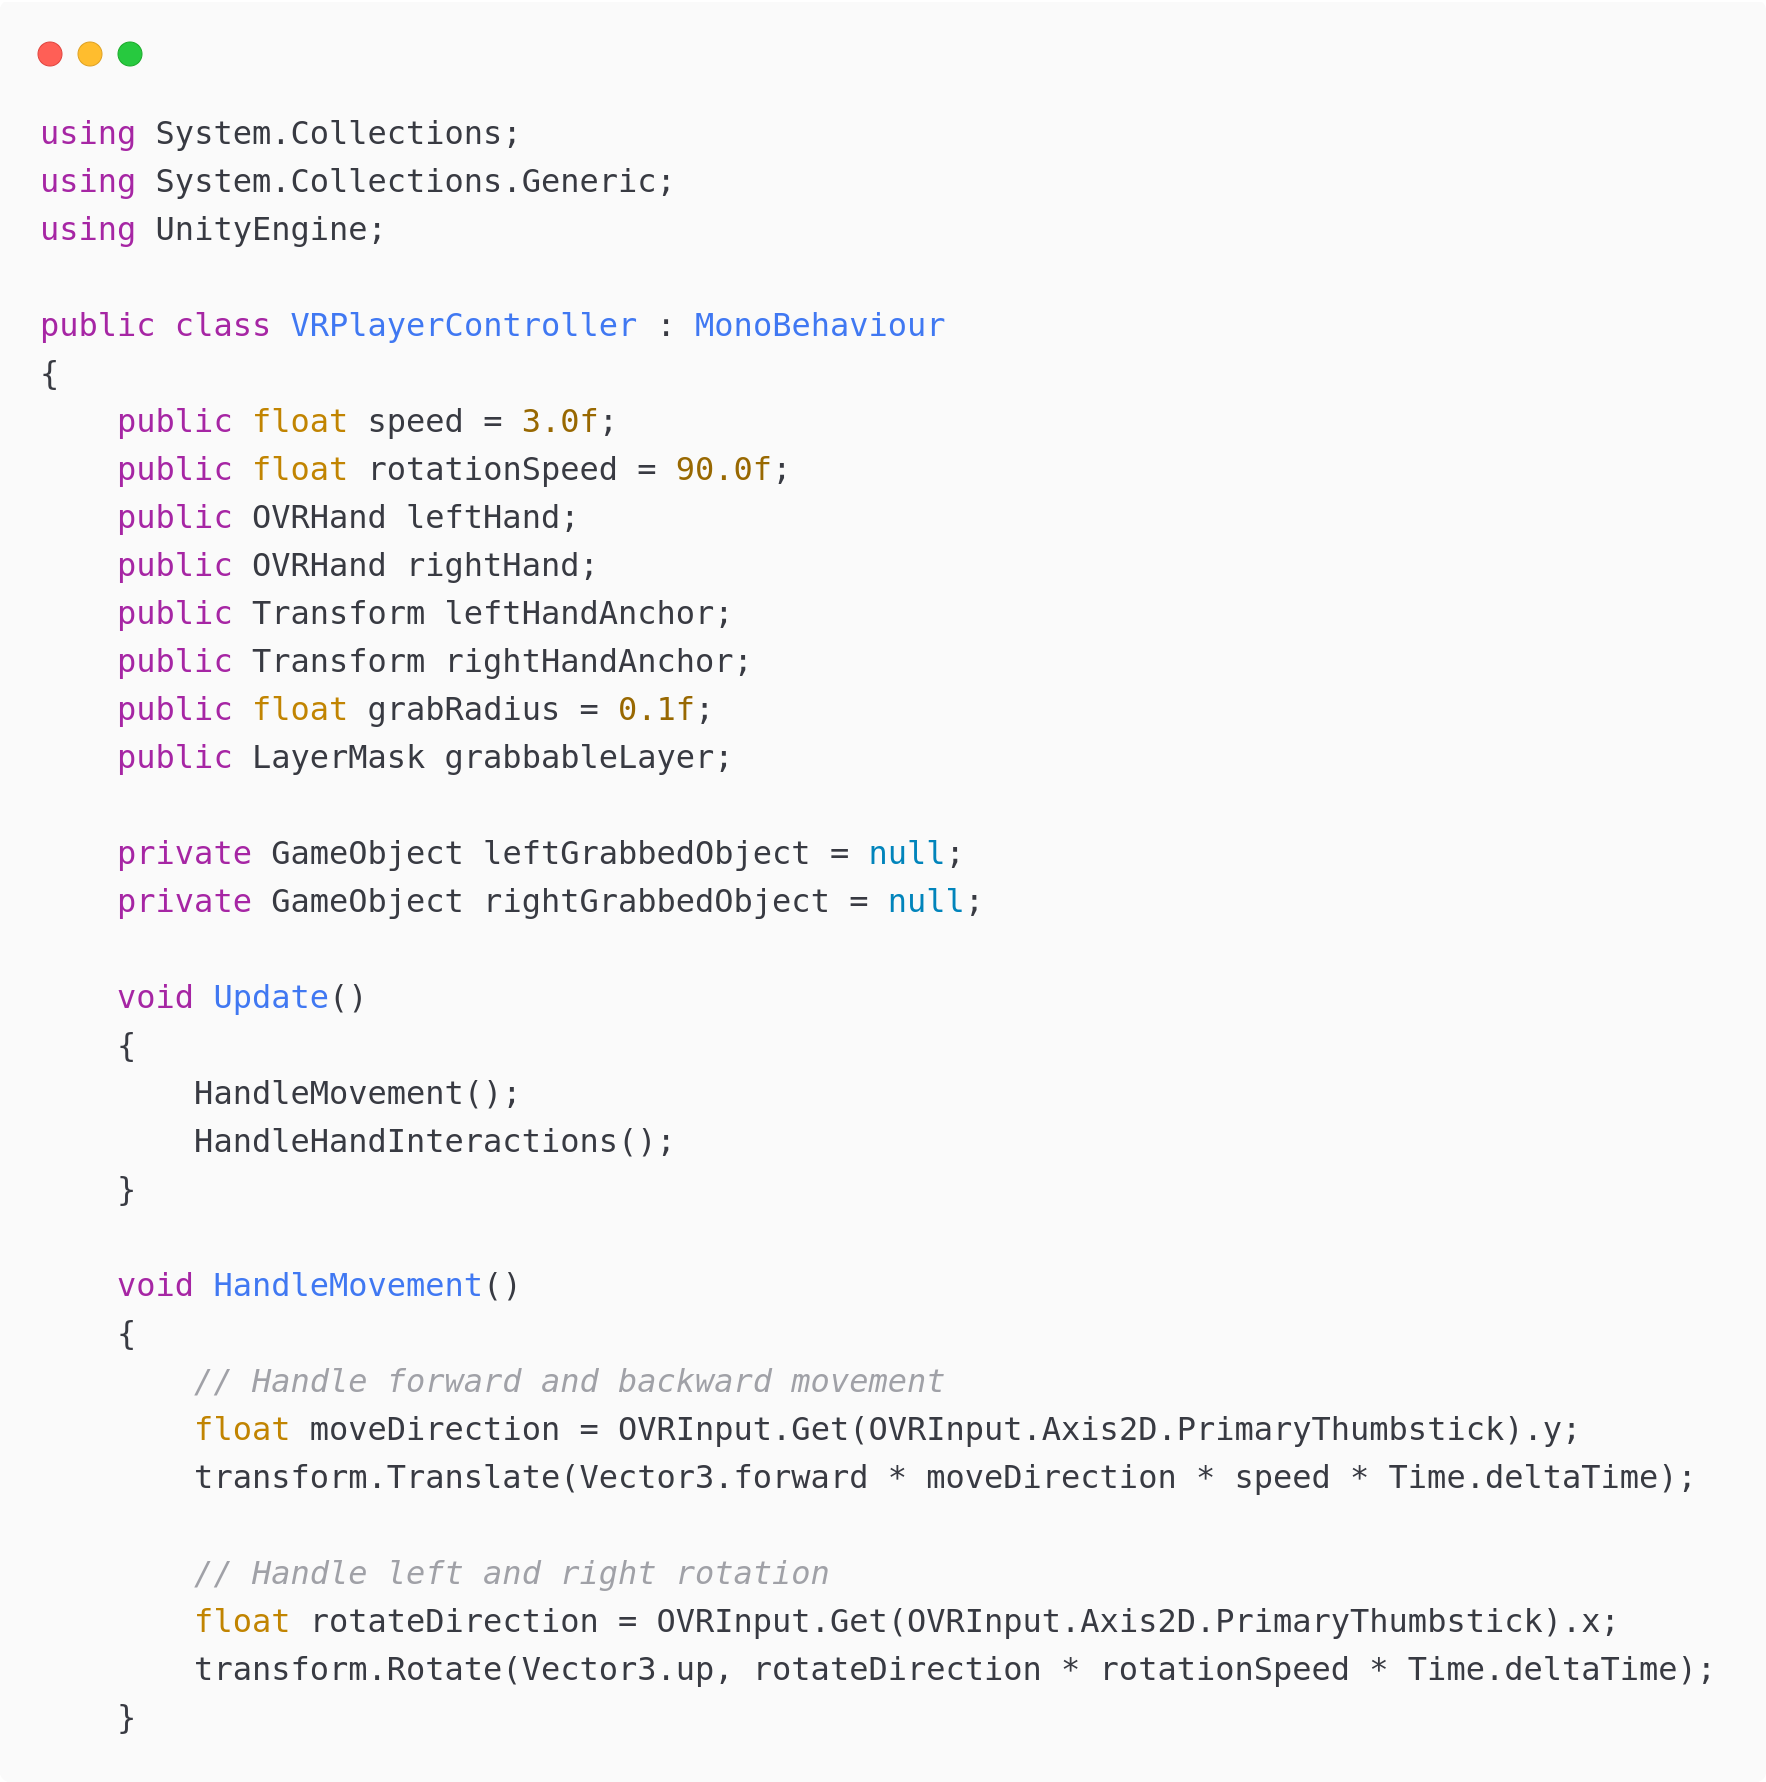
\includegraphics[width=1\textwidth, height=0.7\textheight]{Images/playerp1.png}
	\caption{User Movement Code 1}
	\label{User Movement Code 1}
\end{figure}
\newpage
\text{User movement part 2 code.}
\newline
\begin{figure}[h] 
	\centering
	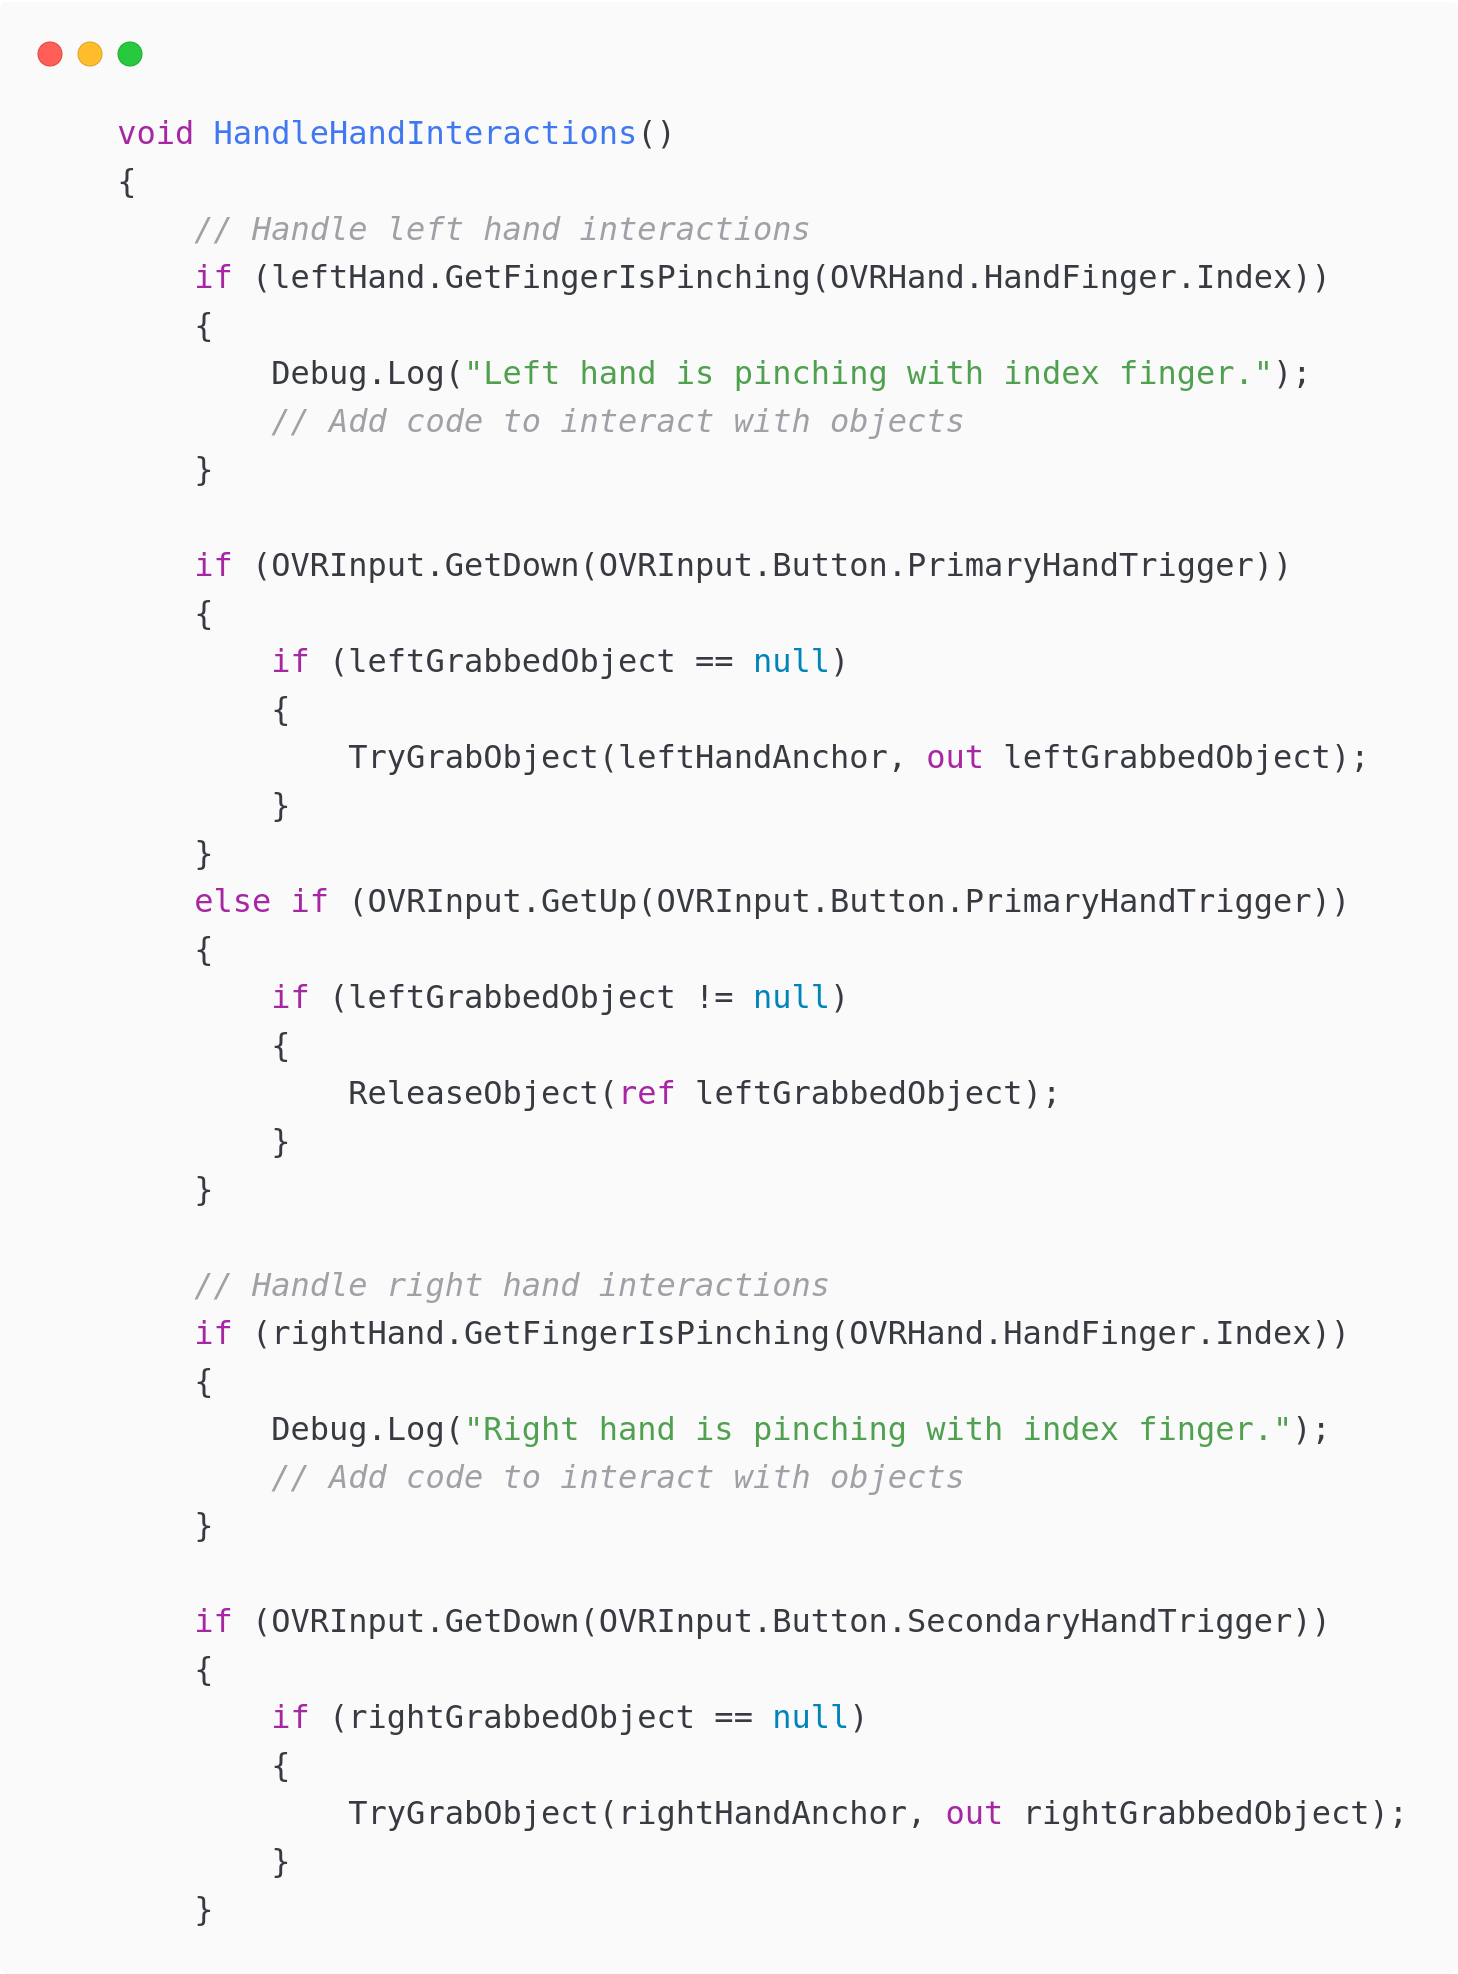
\includegraphics[width=1\textwidth, height=0.7\textheight]{Images/playerp2.png}
	\caption{User Movement Code 2}
	\label{fig:User Movement Code 2}
\end{figure}
\newpage
\text{User movement part 3 code.}
\newline
\begin{figure}[h] 
	\centering
	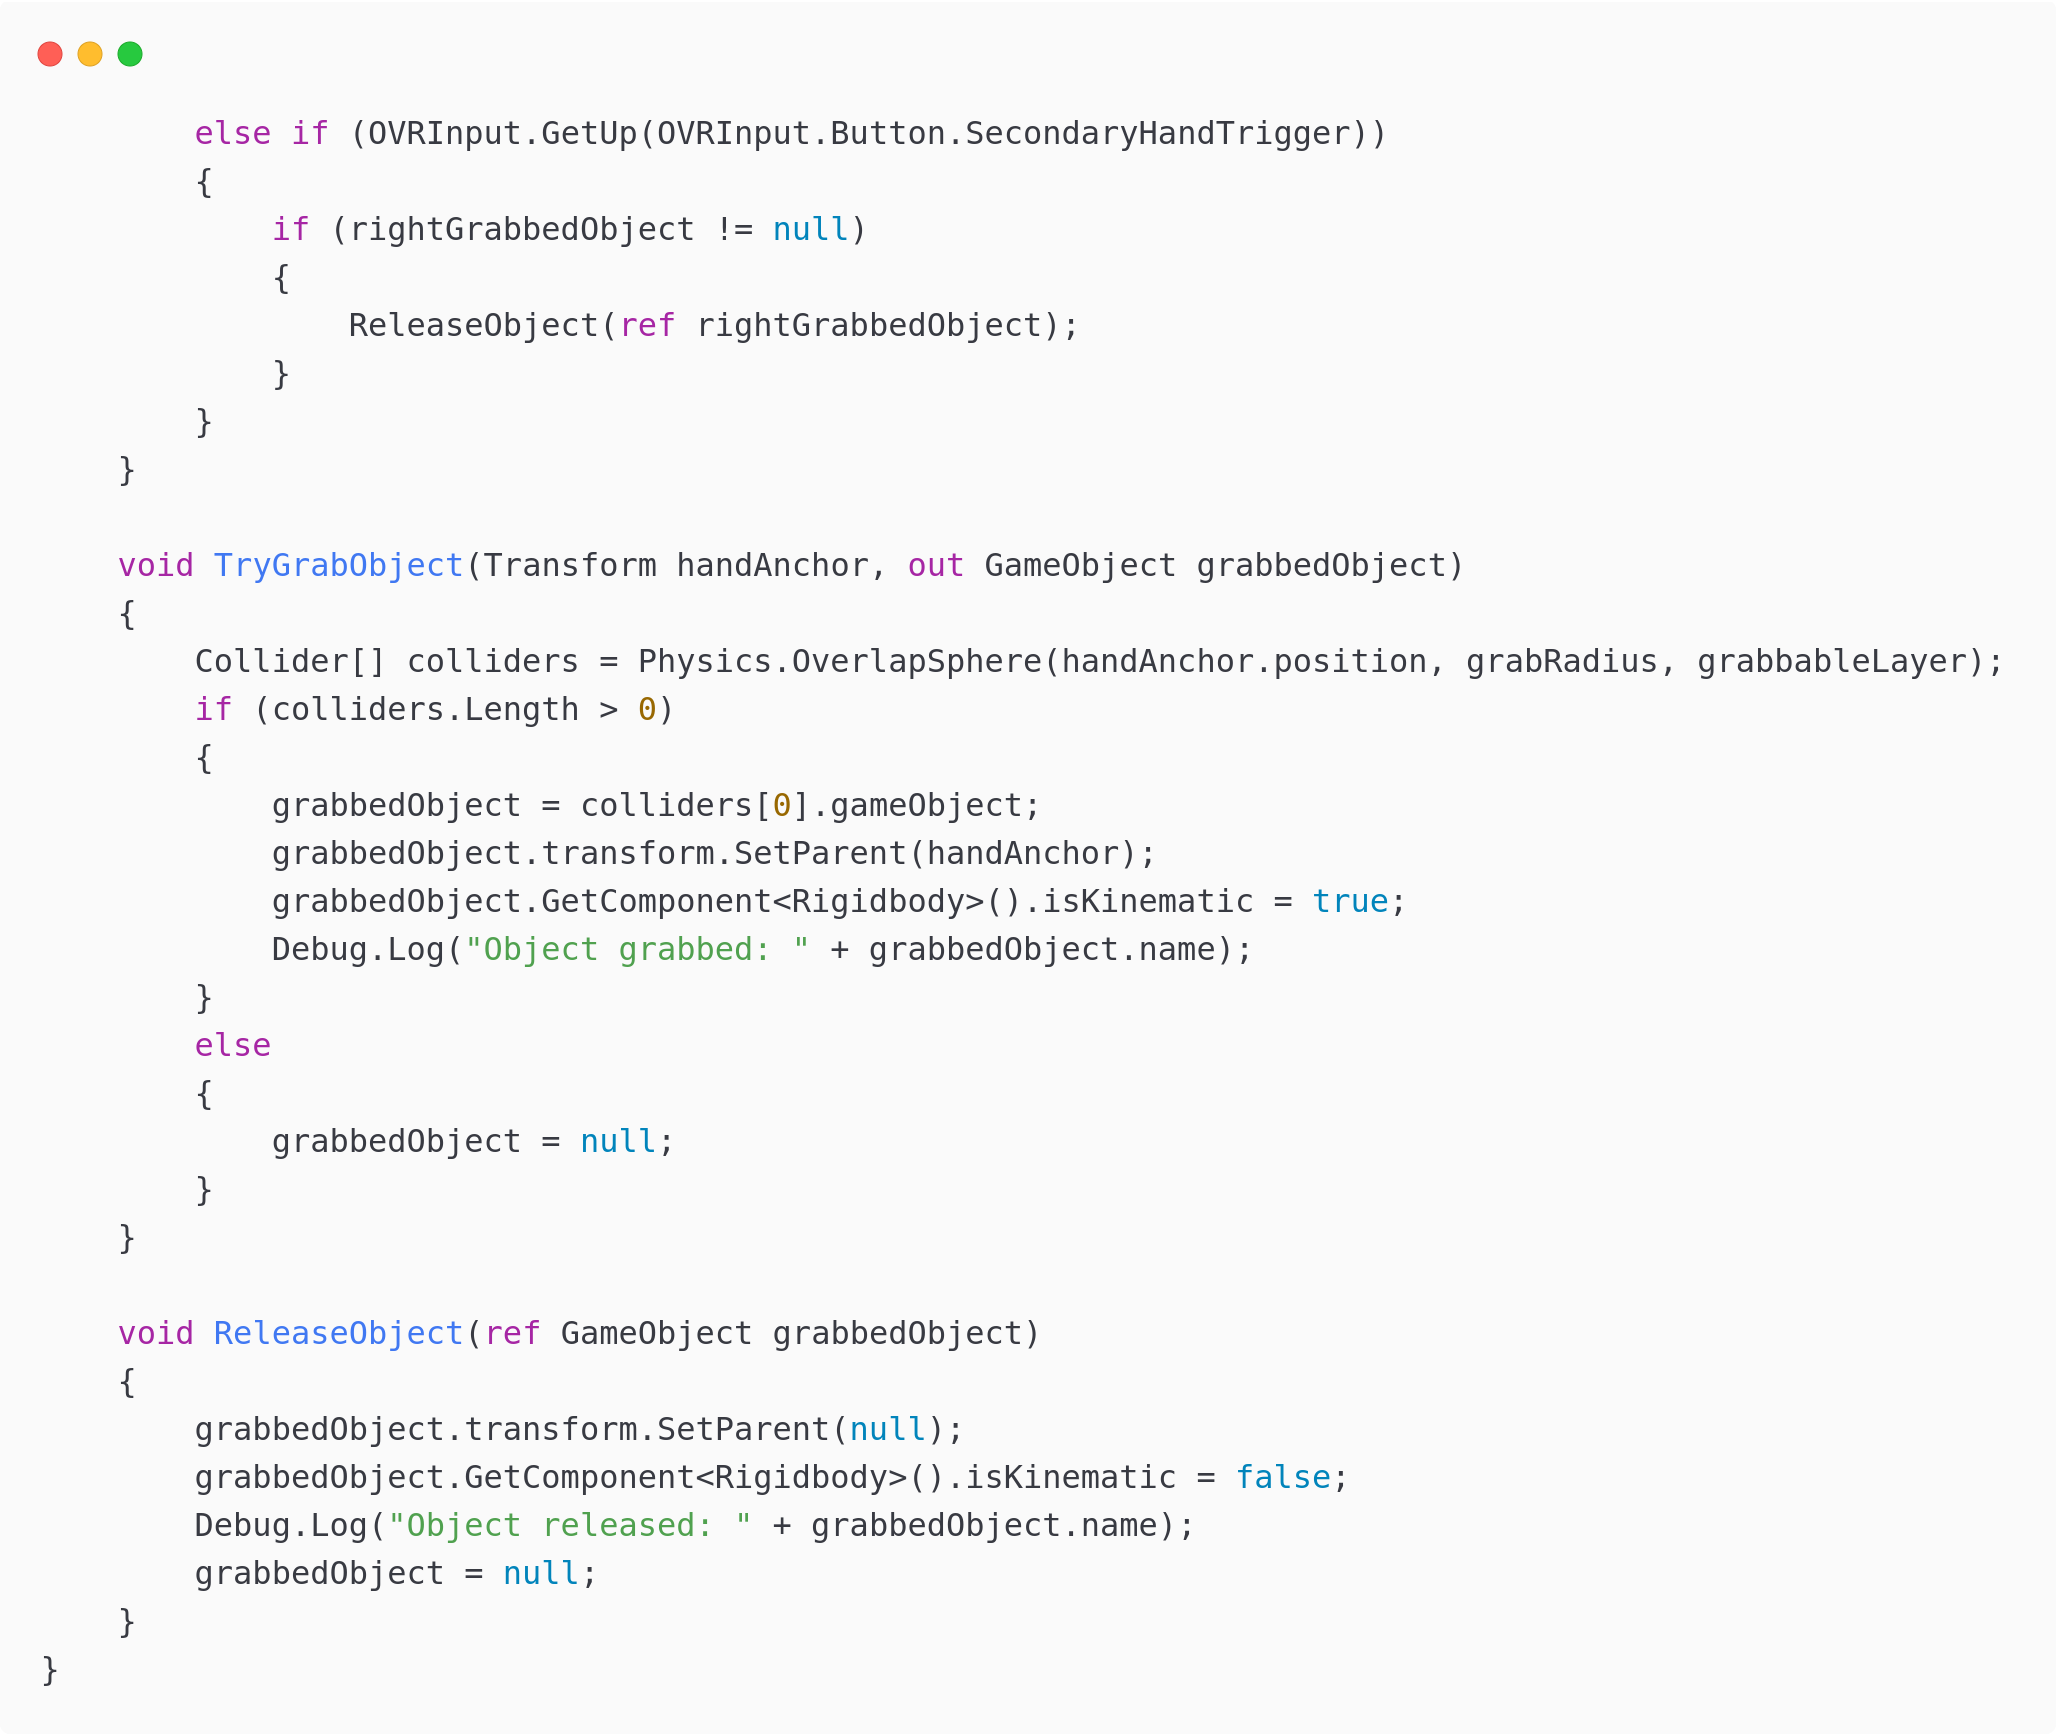
\includegraphics[width=1\textwidth, height=0.7\textheight]{Images/playerp3.png}
	\caption{User Movement Code 3}
	\label{fig:User Movement Code 3}
\end{figure}
\newpage
\text{Code for Pore Alcohol for Hands Washing.}
\newline
\begin{figure}[h]
	\centering
	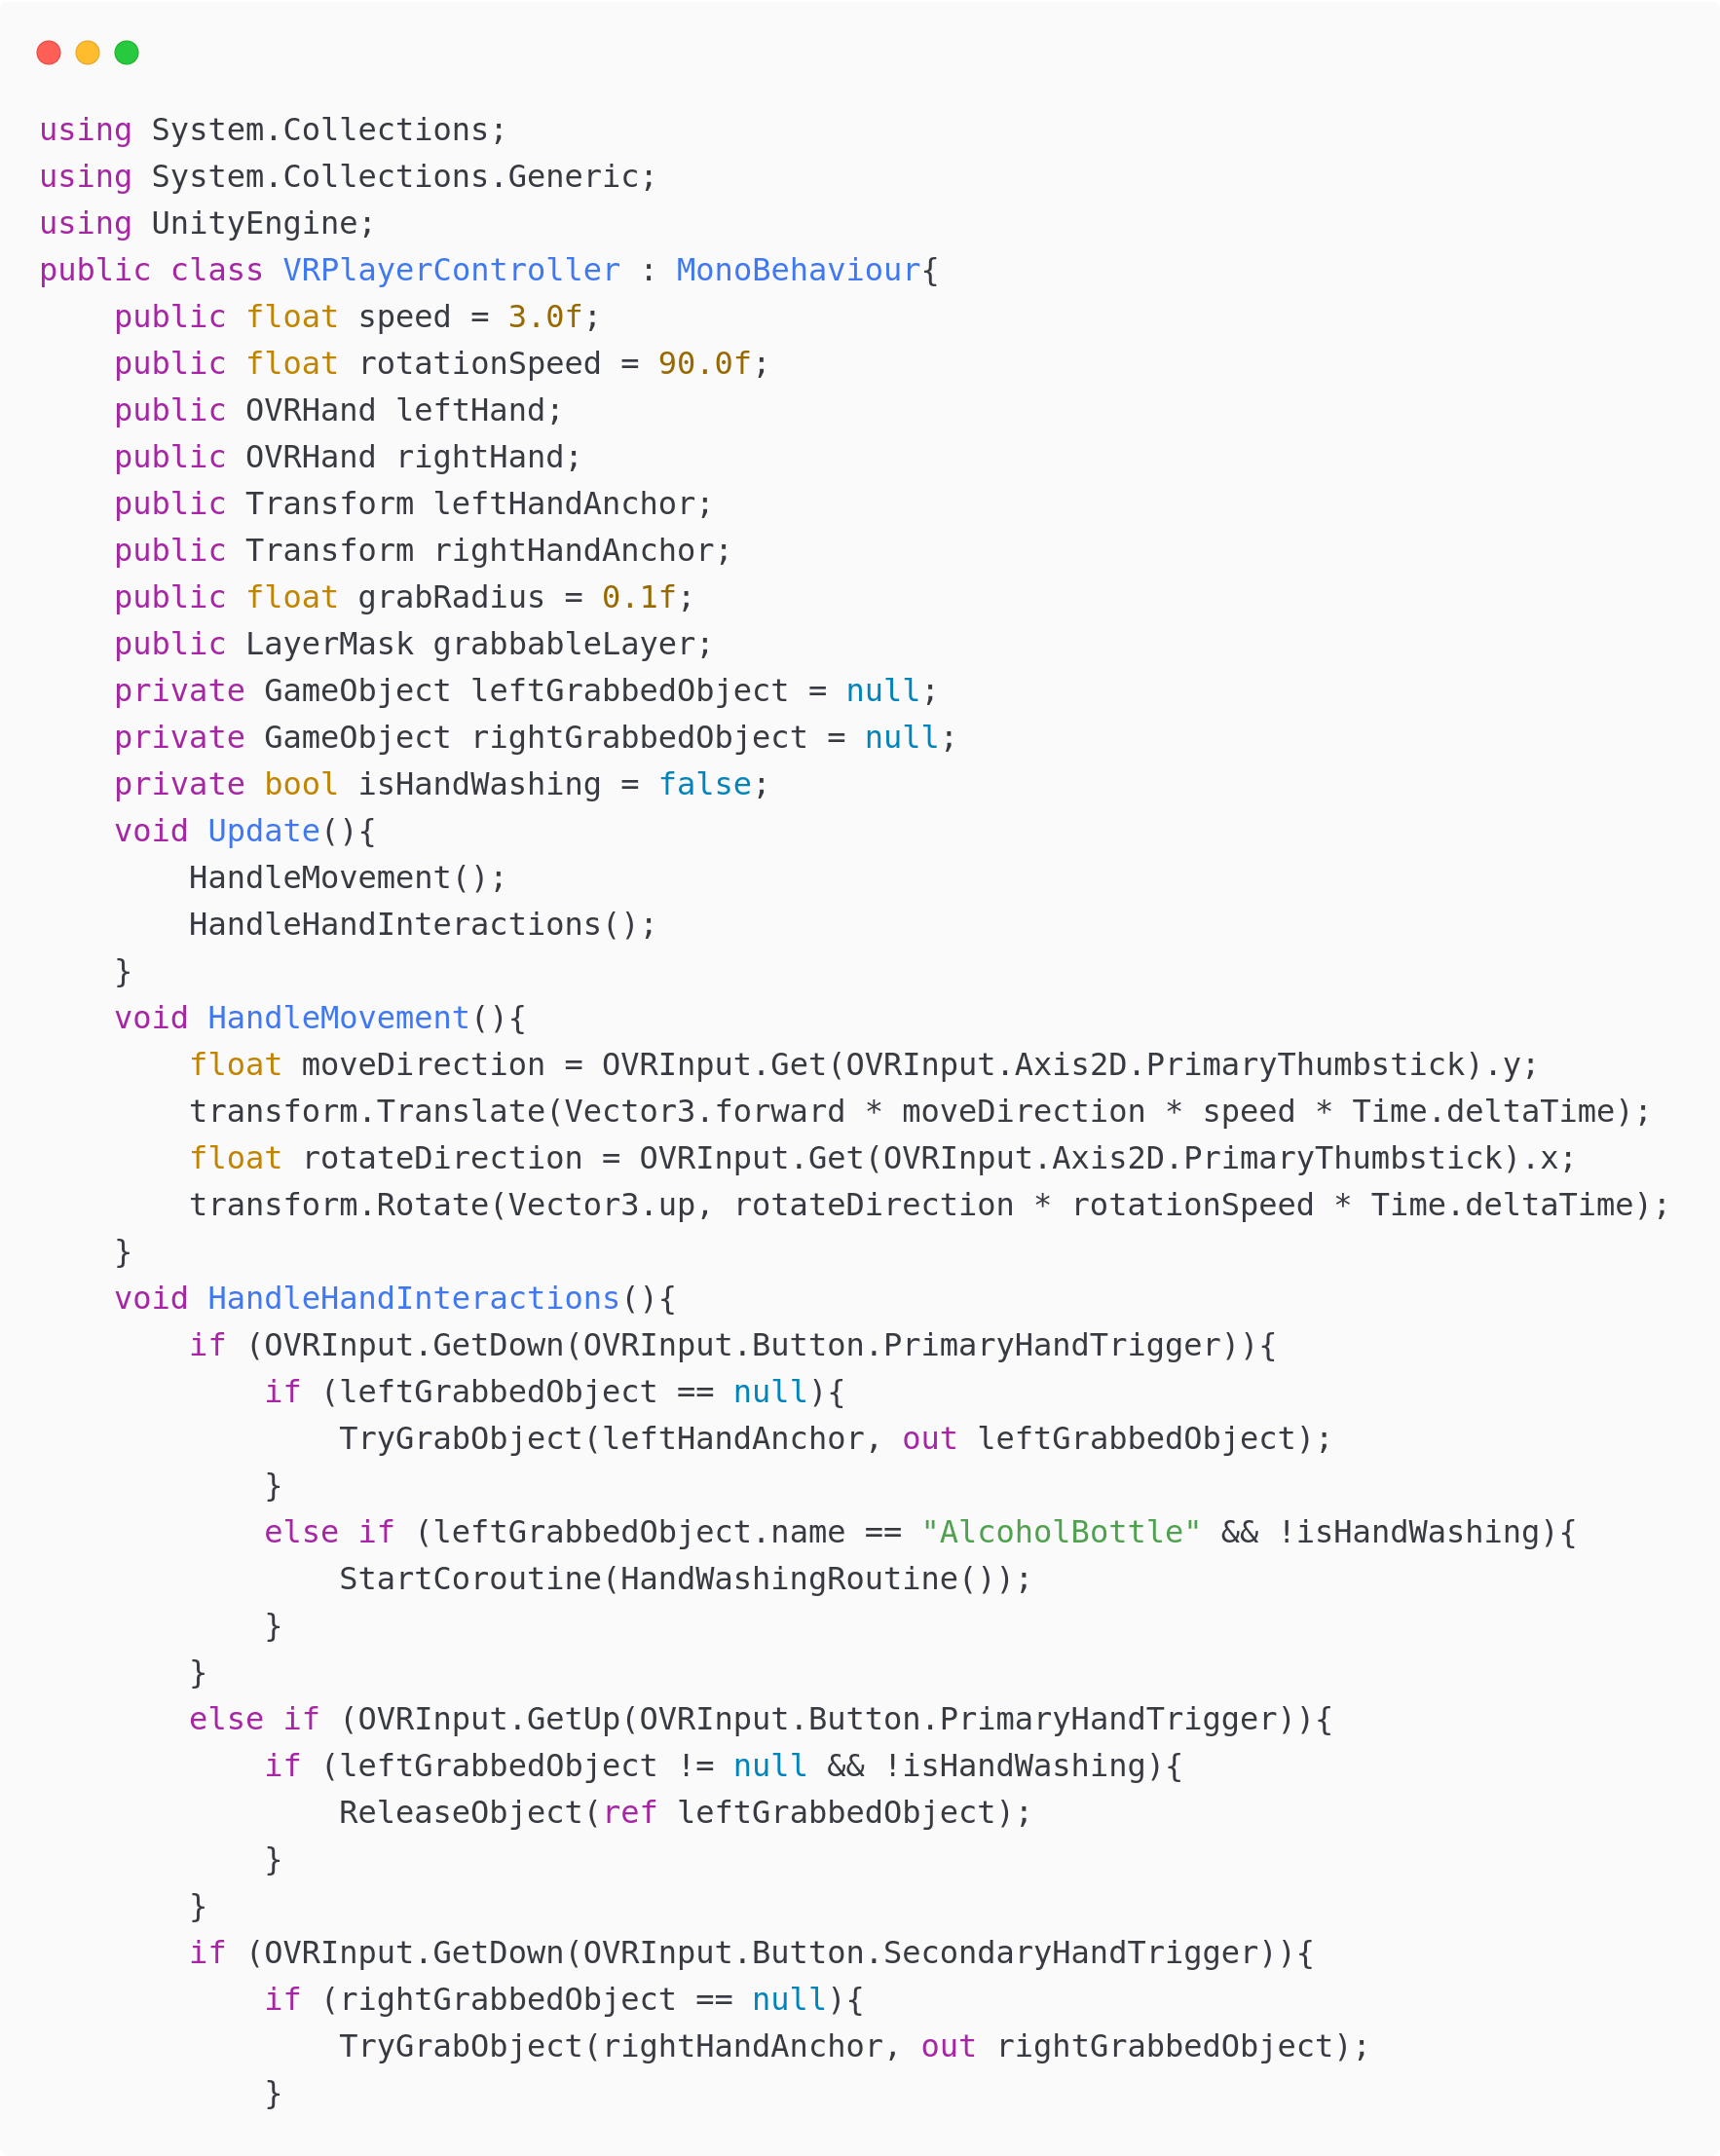
\includegraphics[width=1\textwidth, height=0.7\textheight]{Images/pore alcohol1.png}
	\caption{Pore Alcohol for Hands Washing}
	\label{fig:Grabbing-Tool}
\end{figure}
\newpage
\text{Code for Cleaning Injection Site Part of Body.}
\newline
\begin{figure}[h] 
	\centering
	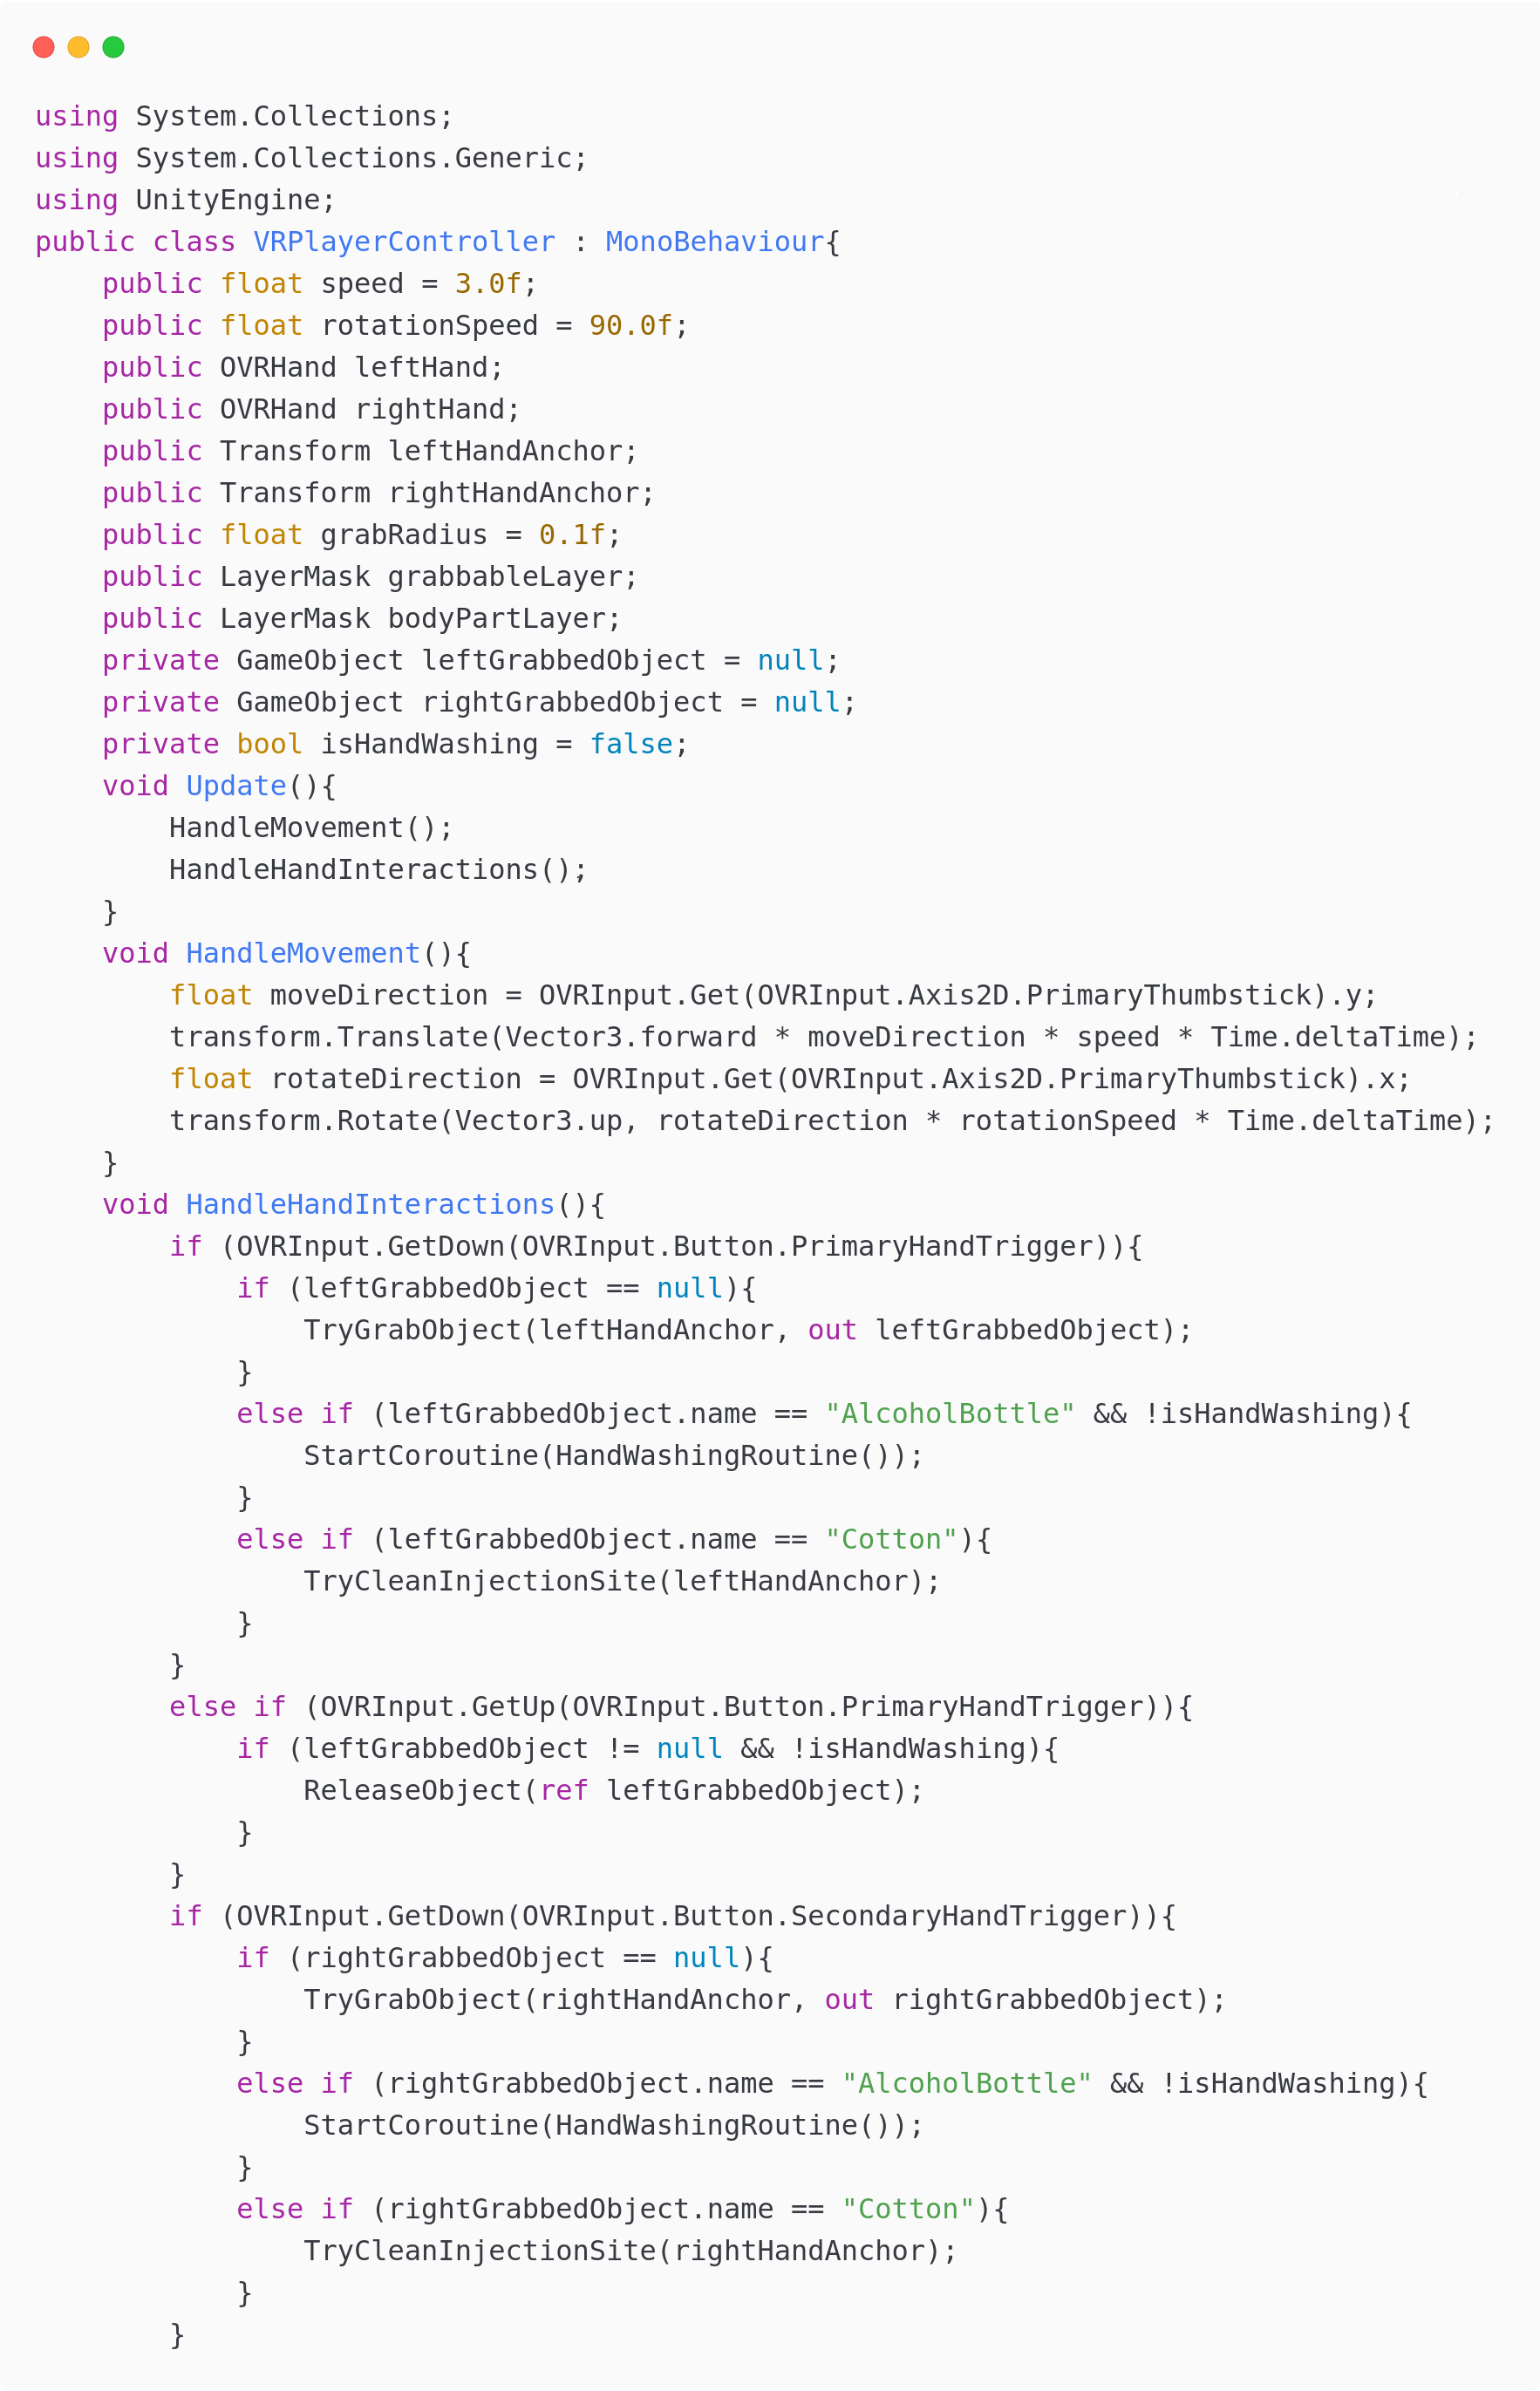
\includegraphics[width=1\textwidth, height=0.7\textheight]{Images/cleaning1.png}
	\caption{Cleaning Injection Site Part}
	\label{fig:Cleaning Injection Site Part}
\end{figure}
\newpage
	\text{ Code for Inject Syringe in Body.}
	\newline
\begin{figure}[h] 
	\centering
	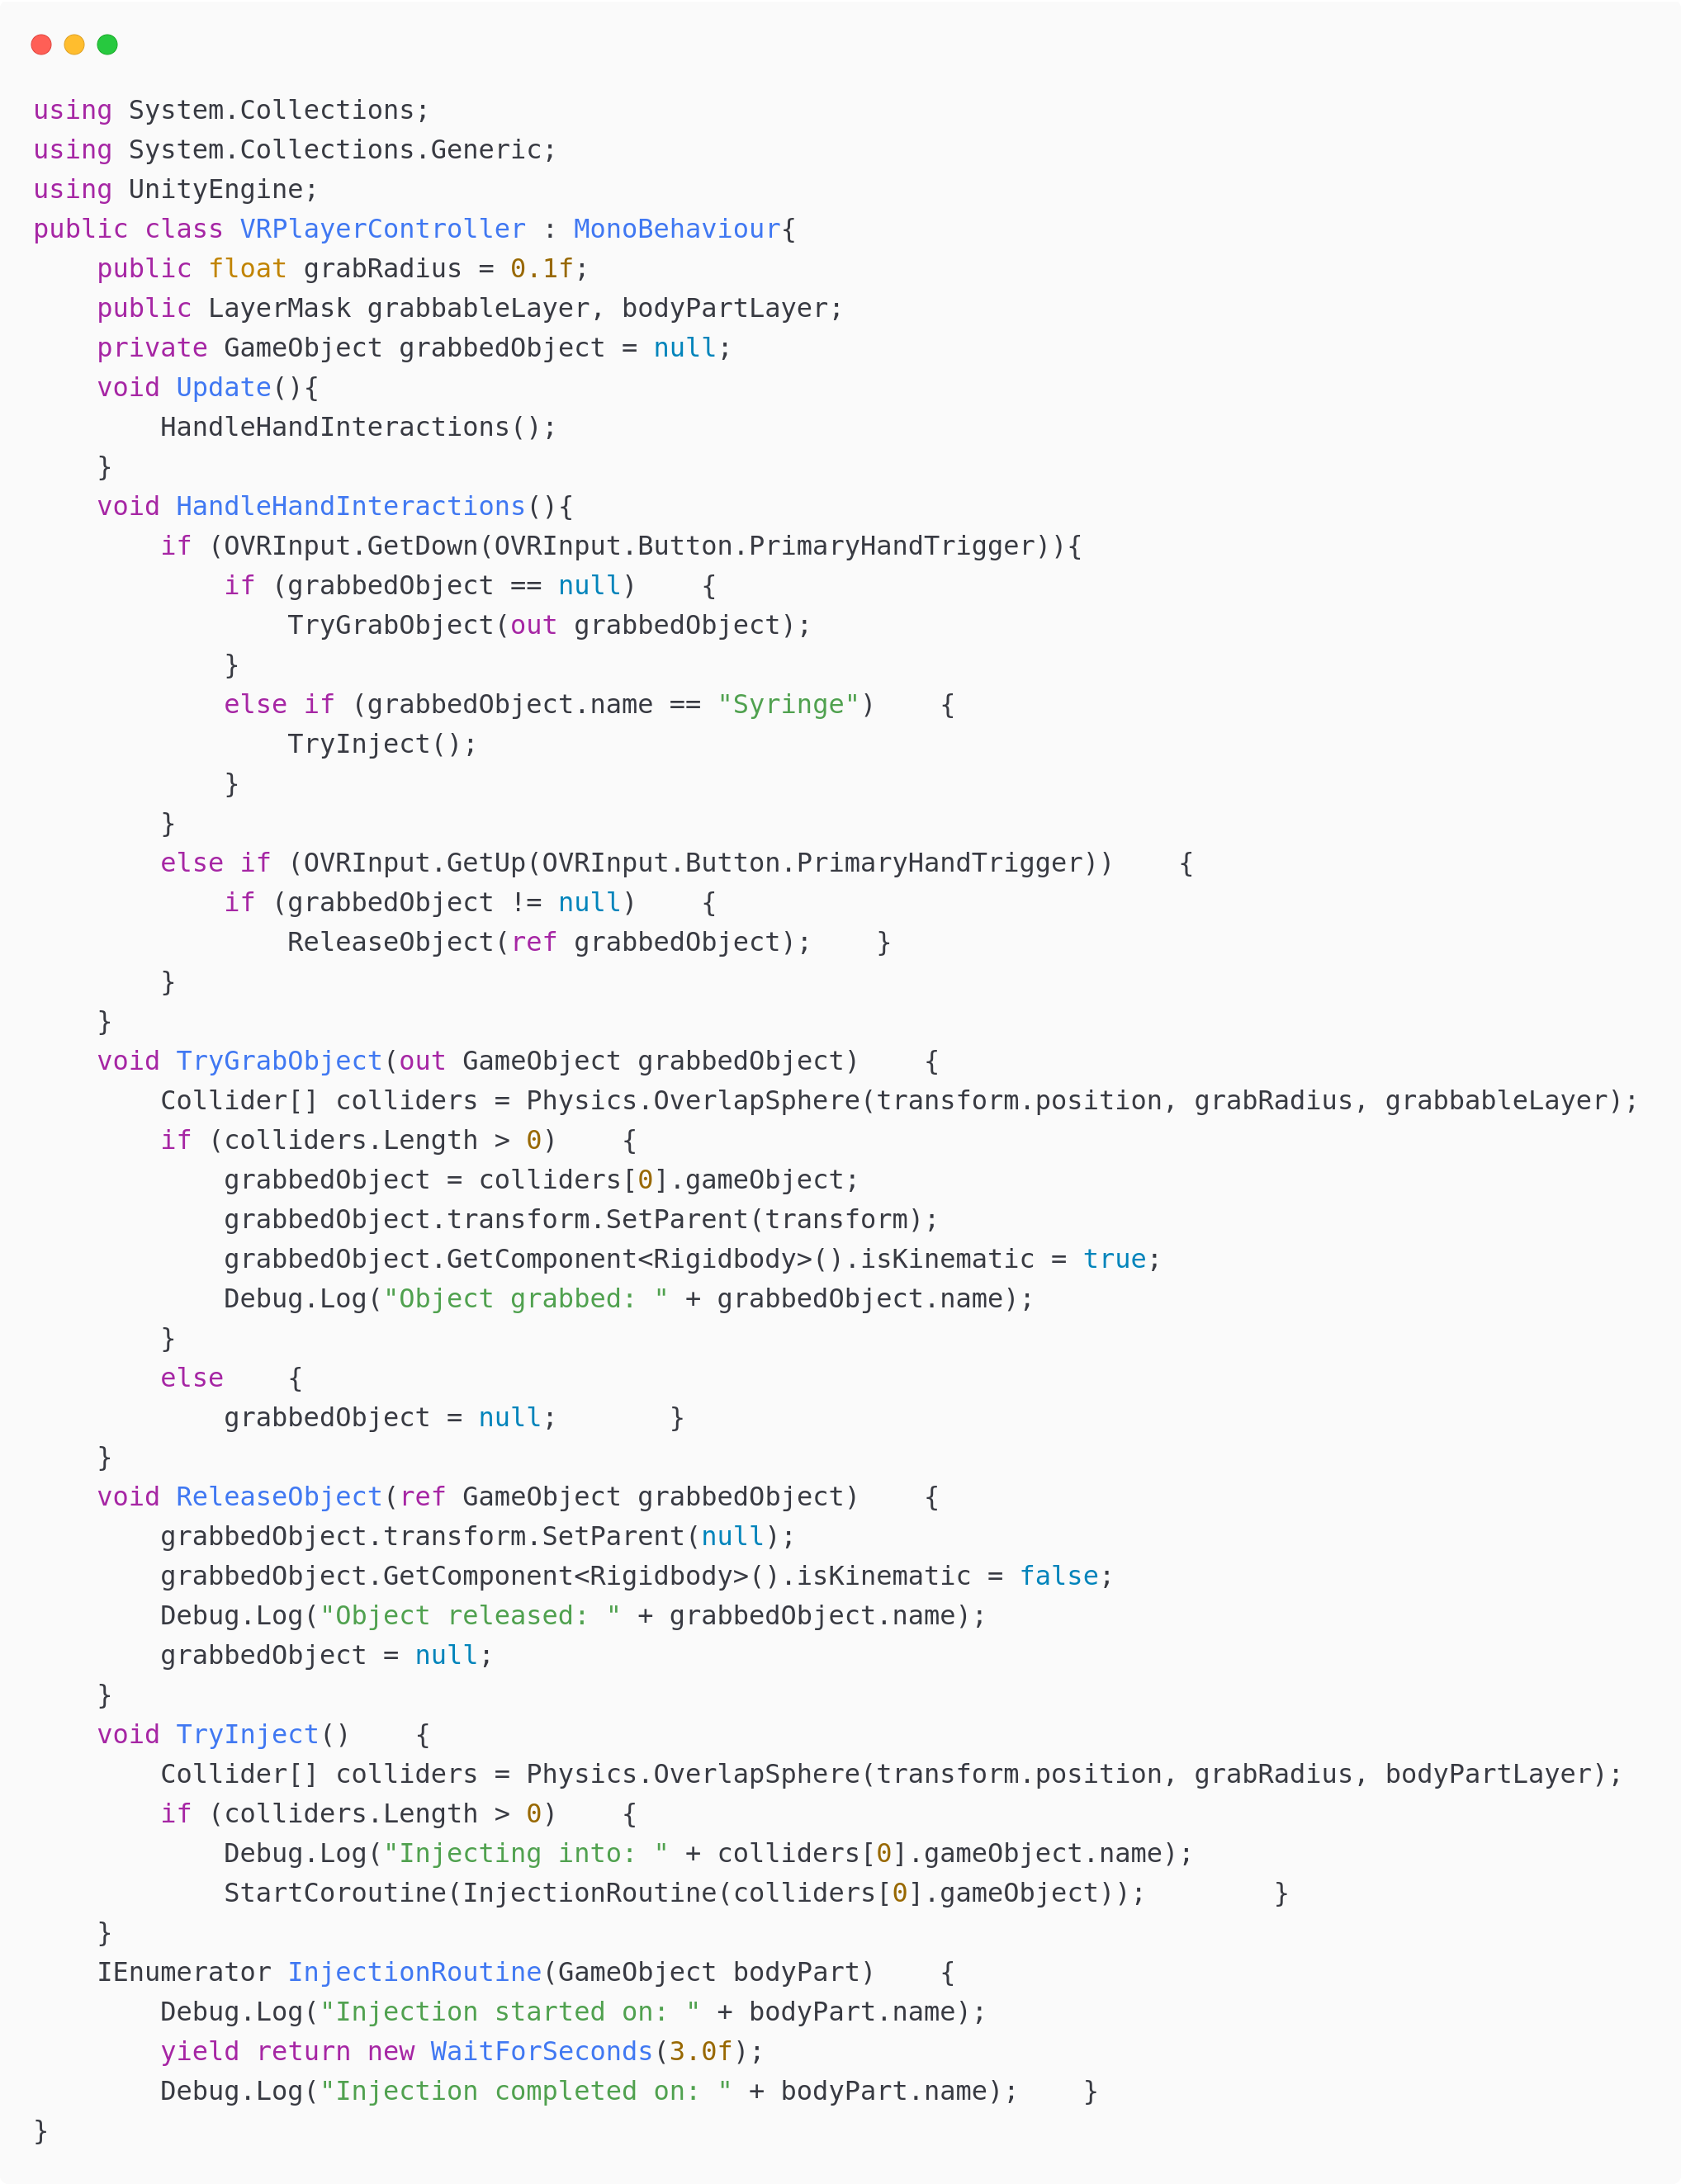
\includegraphics[width=1\textwidth, height=0.7\textheight]{Images/inject syringe.png}
	\caption{Inject Syringe in Body}
	\label{fig:Inject Syringe in Body}
\end{figure}
\newpage
\text{Code for Applying Cut and Bandage on Body.}
\newline
\begin{figure}[h] 
	\centering
	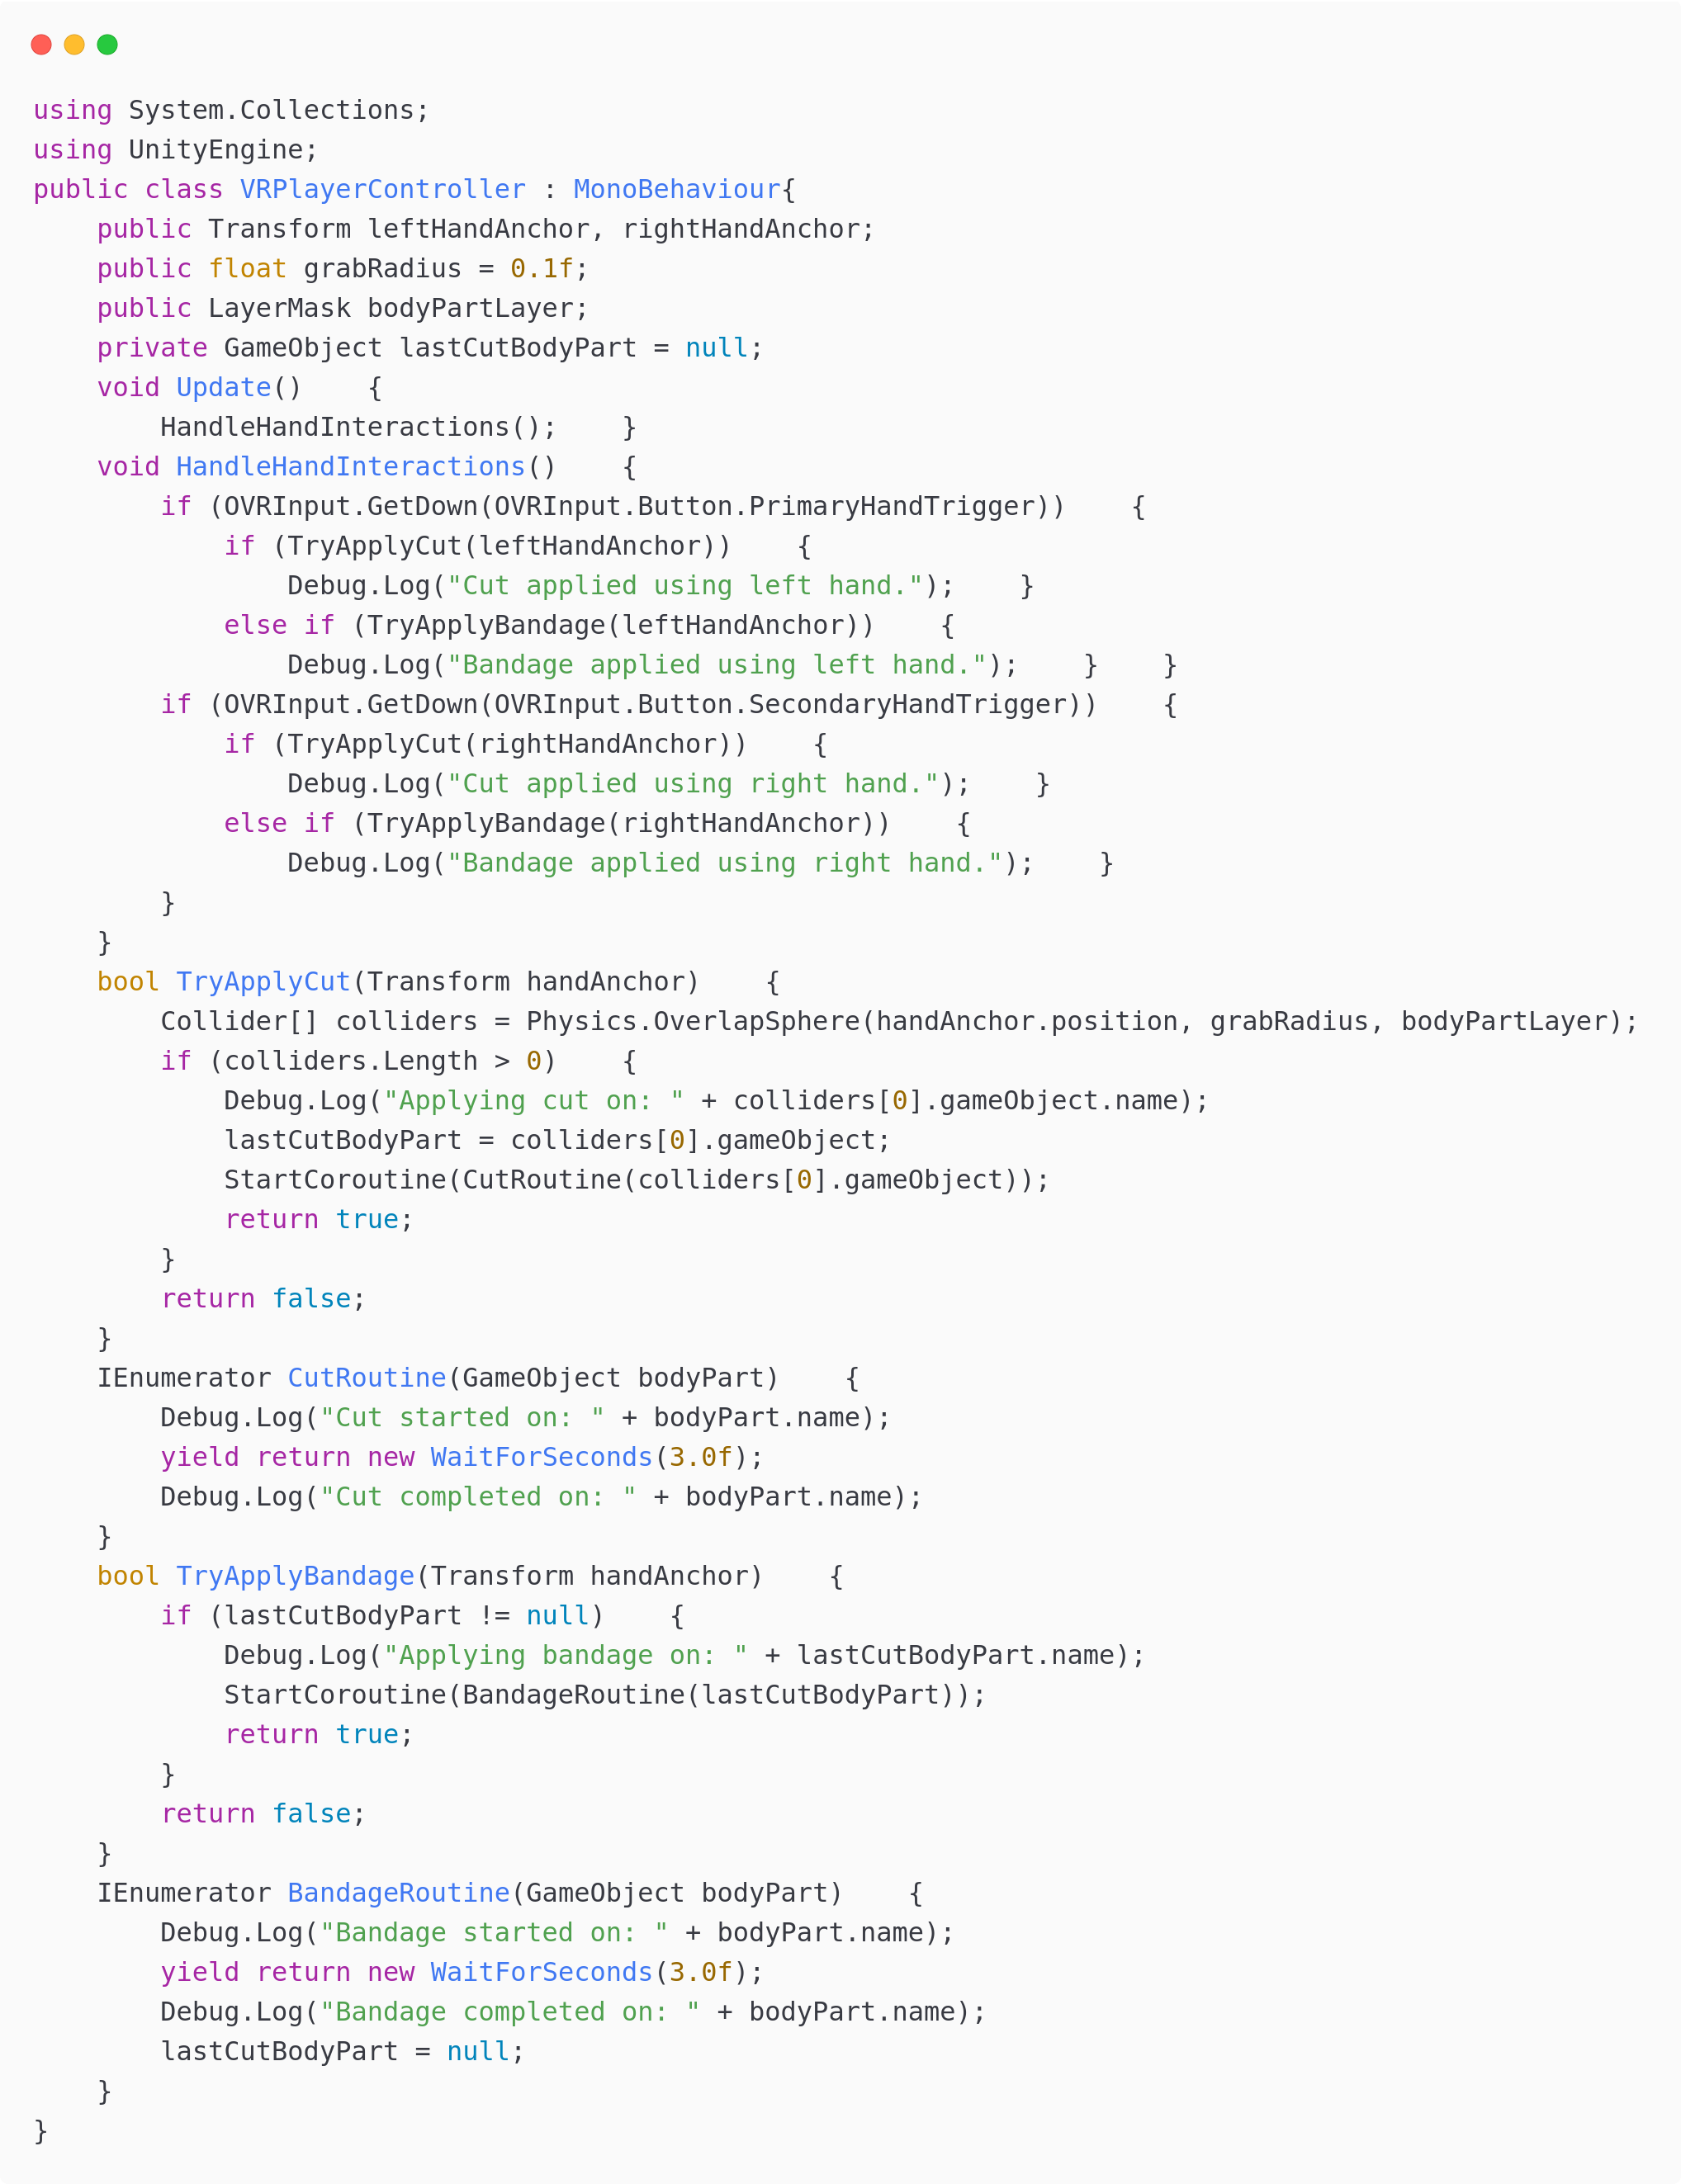
\includegraphics[width=1\textwidth, height=0.7\textheight]{Images/Applying Cut and Bandage on Body.png}
	\caption{Applying Cut and Bandage on Body}
	\label{fig:Applying Cut and Bandage on Body}
\end{figure}
\section{SVN or GitHub}
 Here is the GitHub link: \\
\href{https://github.com/Daudsarfraz/MetaMed}{https://github.com/Daudsarfraz/MetaMed}